\chapter{Prepare the virtual machine}


This chapter explains how to prepare a single virtual machine running
Ubuntu 18.04~LTS amd64 to run TestManager, DLS and a test server.
It means that a single virtual machine will replace the 3 computers
described in Figure \ref{fig:architecture}, because it makes an easier
tutorial.


\section{Creation of the virtual machine}

Create a virtual machine with VirtualBox, with the the following settings:
\begin{itemize}
\item vCPU: 1
\item RAM: 4 GB
\item vDisk: 20 GB
\item Guest OS: Ubuntu 64 bits
\end{itemize}


Download \texttt{ubuntu-18.04-desktop-amd64.iso} from
\url{https://www.ubuntu.com}
and install it in your new virtual machine.

Select a minimum installation with only a web browser and basic utilities
to save disk space.


\subsubsection{Notes}

\begin{itemize}
\item For a very first installation, it is recommended to use exactly the same
  distribution than this guide to avoid any distribution issues.
\item For simplicity, all the components will be installed on the same host,
  but obviously the server and client can run on different machines.
\end{itemize}


\begin{figure}[h!]
  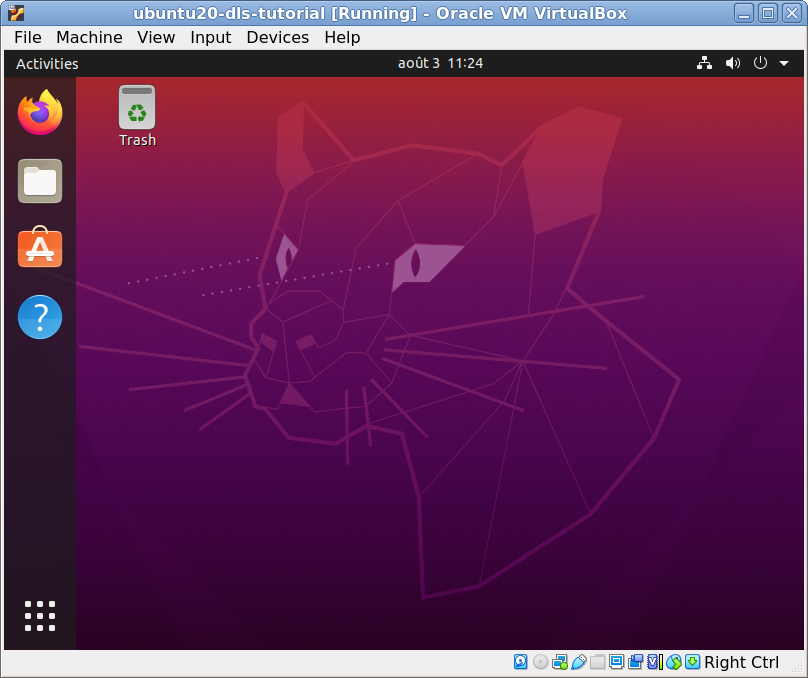
\includegraphics[width=\textwidth]{genpicts/ubuntu-vm.eps}
  \caption{Ubuntu 18.04 LTS amd64 in VirtualBox}
  \label{fig:ubuntu-vm}
\end{figure}
